\documentclass[12pt,fleqn]{article}\usepackage{../../common}
\begin{document}
Ders 1-8

Yaylar ve Agirliklar (Springs and Masses)

Dersimizin uygulama kismina geldik. Diyelim ki alttaki gibi bir yay sistemi var,
4 tane yay 3 tane agirliktan olusuyor, ve sonlari duvar, tavan gibi bir yerde
sabitlenmis.

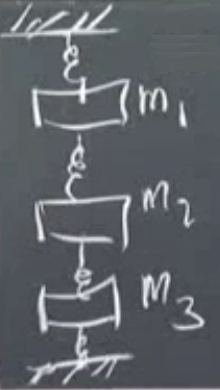
\includegraphics[width=5em]{compscieng_1_08_01.png}

Kutlelerin bir agirligi var tabii, agirliklar o yaylar asagi dogru cekiyor, bu
cekim yaylari acacak, gerecek, soru yaylarin ne kadar asagi inecegi.  Bir yer
degisim (displacement) sorusu bu yani. Unutmayalim yay acilip kapanan bir
mekanizmadir ama acilirken de kapanirken de bir direnc gosterir. Yer degisim en
ustte ve en altta sifir cunku oralar sabitlenmis.

Bir baslangic hali dusunursek, diyelim ki yercekimi o anda etkisiz, ama sonra
yercekimini bir dugmeye basip aciyoruz, her yay baslangic halinden asagi
dogru bir yer degisimi yasayacak, 

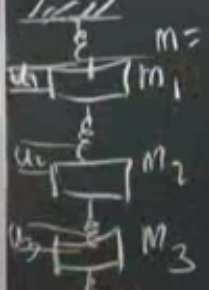
\includegraphics[width=5em]{compscieng_1_08_02.png}

bunlara $u_1,u_2,u_3$ diyebiliriz.

Dikkat salinimi olcmeye ugrasmiyoruz burada, o daha sonraki derslerde devreye
girecek, zaman faktorunu resme dahil edecegiz, o sonra. Simdi sadece kalici
durumla ilgileniyorum, yercekimi aciliyor, yaylar asagi dogru uzuyor, ve her sey
yerli yerine oturduktan sonra gozlemlenecek yer degisimiyle ilgileniyorum su
anda.

Her yay parcasinin ne kadar uzadigi / esnedigi (elongation) ayri bir olcut.
Dusunursek ikinci kutledeki yer degisimi $u_2$ icinde hem ikinci hem de birinci
yayin esnemesi rol oynar. O yuzden esneme icin ayri bir degisken kullaniyoruz,
$e_1,e_2,e_3$. O zaman kinci yay ne kadar uzar? $u_2-u_1$ kadar. Bir farktan
bahsediyoruz burada. Bazi yaylar sikisma da yasayabilir tabii, mesela tahmin
ediyorum ki en alttaki yayda sikisma olacak.

Tum bunlar isin geometrik kismi bir anlamda, yer, uzama, kisalma.. Materyel
faktorlere resme dahil etmek lazim, Hooke Kanunu bunu yapacak. Ilk agirlik
mesela asagi inerken ilk yayi gerecek. Hooke Kanunu bu noktada der ki yay belli
bir kuvvetle agirligi geri cekecek, bu cekis yayin gerilmesi / uzamasiyla
orantili olacak. Her yaydaki kuvvete $w_1,w_2,w_3,w_4$ diyelim. Esneme ile ona
karsilik ortaya cikan kuvvet iliskisi her materyel icin farkli olur, materyele
gore, yay cesidini gore degisen Hooke yay sabiti bu farkliligi denkleme dahil
edebilir, bu sabitlere $c_1,c_2,c_3,c_4$ diyelim.

Hooke Kanunun lineerdir, ki asiri fazla olmayan esnemeler icin lineerlik
gecerli olacaktir, muhakkak yayi asiri gerseydik belli bir noktadan sonra
lineer olmayan etkiler gorebilirdik, biz bu tur asiri sonuclara su anda
bakmiyoruz.

Devam edelim, Hooke Kanunu der ki her yaydaki kuvvet o yaydaki esnemeyle orantilidir,

$$
w_i = c_i e_i 
$$

Burada bir kosegen matris goruyorum ben, tum yaylar, esnemeler, sabitler icin

$$
\left[\begin{array}{c}
w_1 \\ w_2 \\ w_3 \\ w_4
\end{array}\right] =
\left[\begin{array}{cccc}
c_1 & & & \\  & c_2 & & \\  & & c_3 & \\ & & & c_4
\end{array}\right]
\left[\begin{array}{c}
e_1 \\ e_2 \\ e_3 \\ e_4
\end{array}\right] 
$$

Ve nihai matris formunda

$$
w = C e
$$

ki $w,C,e$ ustte gorulen vektorler ve matris. Materyel kismi bu sekilde dahil
etmis olduk, ortadaki sabit matrisi uzerinden. Benzer kanunlar fizigin diger
kisimlarinda da gorulebilir, mesela ustteki $C$ matrisi iletkenligi de temsil
ediyor olabilirdi. Demek istedigim materyel ozellikleri denkleme oradan dahil
oluyor. Bu resmi nasil tamamlariz? Yercekim bir dis kuvvet, kutleler var, yer
degisimlerine sebep oluyor..

Resmi tamamlamak icin ``kuvvet denge'' denklemi ekleyecegim, her kutle
icin bir denge denklemi olacak.

Not ekleyelim, ustteki turden problem modellemesi pek cok diger uygulamada ise
yariyor. Bir geometri var, buradan bir $A$ matrisi cikartiyoruz, sonra bir
fiziksel adim var, oradan $C$ matrisi geliyor, ve kuvvet dengesi ekleniyor,
resim tamamlaniyor. Kuvvet denge denklemi diger bir alanda, mesela elektrikte,
Kirchoff Akim Kanunu olabilirdi, ileride ag yapilarina bakarken gorecegiz, giren
akim cikan akima esit.. Buradaki denge bir yandaki kuvvetin diger yandakine esit
olmasi. Eger sistemde bir dengeden (equilibrium) bahsedebiliyorsak bir denge
denklemi yazabiliriz demektir.

Simdi esneme kismini matris formuna cevirelim. Ne demistik? Mesela ikinci yay
esnemesi ikinci yer degisimi eksi birinci yer degisimi. Matrissel formda
konusmak icin $e_i$ ve $u_j$  vektorlere lazim, iliskileri bir matris carpimi.
Alttaki matriste ikinci satira ne yazariz?

$$
\left[\begin{array}{c}
e_1 \\ e_2 \\ e_3 \\ e_4
\end{array}\right] =
\left[\begin{array}{cccc}
 & & \\ ? & ? & ? \\  & & \\  & & 
\end{array}\right]
\left[\begin{array}{c}
u_1 \\ u_2 \\ u_3 
\end{array}\right]
$$

O satir sagdaki $u$ vektoru ile carpilip sonuclari toplanacak, o zaman
$u_1$ eksi bir ile, $u_2$ arti bir ile carpilir, $u_3$ ile ilgilenmiyoruz,
orasi sifir, yani

$$
\left[\begin{array}{c}
e_1 \\ e_2 \\ e_3 \\ e_4
\end{array}\right] =
\left[\begin{array}{cccc}
 & & \\ -1 & 1 & 0 \\  & & \\  & & 
\end{array}\right]
\left[\begin{array}{c}
u_1 \\ u_2 \\ u_3 
\end{array}\right]
$$




















[devam edecek]

\end{document}
